% Options for packages loaded elsewhere
\PassOptionsToPackage{unicode}{hyperref}
\PassOptionsToPackage{hyphens}{url}
%
\documentclass[
]{article}
\usepackage{lmodern}
\usepackage{amssymb,amsmath}
\usepackage{ifxetex,ifluatex}
\ifnum 0\ifxetex 1\fi\ifluatex 1\fi=0 % if pdftex
  \usepackage[T1]{fontenc}
  \usepackage[utf8]{inputenc}
  \usepackage{textcomp} % provide euro and other symbols
\else % if luatex or xetex
  \usepackage{unicode-math}
  \defaultfontfeatures{Scale=MatchLowercase}
  \defaultfontfeatures[\rmfamily]{Ligatures=TeX,Scale=1}
\fi
% Use upquote if available, for straight quotes in verbatim environments
\IfFileExists{upquote.sty}{\usepackage{upquote}}{}
\IfFileExists{microtype.sty}{% use microtype if available
  \usepackage[]{microtype}
  \UseMicrotypeSet[protrusion]{basicmath} % disable protrusion for tt fonts
}{}
\makeatletter
\@ifundefined{KOMAClassName}{% if non-KOMA class
  \IfFileExists{parskip.sty}{%
    \usepackage{parskip}
  }{% else
    \setlength{\parindent}{0pt}
    \setlength{\parskip}{6pt plus 2pt minus 1pt}}
}{% if KOMA class
  \KOMAoptions{parskip=half}}
\makeatother
\usepackage{xcolor}
\IfFileExists{xurl.sty}{\usepackage{xurl}}{} % add URL line breaks if available
\IfFileExists{bookmark.sty}{\usepackage{bookmark}}{\usepackage{hyperref}}
\hypersetup{
  pdftitle={Klk\_Genes\_Data\_Analysis},
  pdfauthor={Anouk Dupe, Maria Yemane, Dustin Schilling, David Eckey},
  hidelinks,
  pdfcreator={LaTeX via pandoc}}
\urlstyle{same} % disable monospaced font for URLs
\usepackage[margin=1in]{geometry}
\usepackage{color}
\usepackage{fancyvrb}
\newcommand{\VerbBar}{|}
\newcommand{\VERB}{\Verb[commandchars=\\\{\}]}
\DefineVerbatimEnvironment{Highlighting}{Verbatim}{commandchars=\\\{\}}
% Add ',fontsize=\small' for more characters per line
\usepackage{framed}
\definecolor{shadecolor}{RGB}{248,248,248}
\newenvironment{Shaded}{\begin{snugshade}}{\end{snugshade}}
\newcommand{\AlertTok}[1]{\textcolor[rgb]{0.94,0.16,0.16}{#1}}
\newcommand{\AnnotationTok}[1]{\textcolor[rgb]{0.56,0.35,0.01}{\textbf{\textit{#1}}}}
\newcommand{\AttributeTok}[1]{\textcolor[rgb]{0.77,0.63,0.00}{#1}}
\newcommand{\BaseNTok}[1]{\textcolor[rgb]{0.00,0.00,0.81}{#1}}
\newcommand{\BuiltInTok}[1]{#1}
\newcommand{\CharTok}[1]{\textcolor[rgb]{0.31,0.60,0.02}{#1}}
\newcommand{\CommentTok}[1]{\textcolor[rgb]{0.56,0.35,0.01}{\textit{#1}}}
\newcommand{\CommentVarTok}[1]{\textcolor[rgb]{0.56,0.35,0.01}{\textbf{\textit{#1}}}}
\newcommand{\ConstantTok}[1]{\textcolor[rgb]{0.00,0.00,0.00}{#1}}
\newcommand{\ControlFlowTok}[1]{\textcolor[rgb]{0.13,0.29,0.53}{\textbf{#1}}}
\newcommand{\DataTypeTok}[1]{\textcolor[rgb]{0.13,0.29,0.53}{#1}}
\newcommand{\DecValTok}[1]{\textcolor[rgb]{0.00,0.00,0.81}{#1}}
\newcommand{\DocumentationTok}[1]{\textcolor[rgb]{0.56,0.35,0.01}{\textbf{\textit{#1}}}}
\newcommand{\ErrorTok}[1]{\textcolor[rgb]{0.64,0.00,0.00}{\textbf{#1}}}
\newcommand{\ExtensionTok}[1]{#1}
\newcommand{\FloatTok}[1]{\textcolor[rgb]{0.00,0.00,0.81}{#1}}
\newcommand{\FunctionTok}[1]{\textcolor[rgb]{0.00,0.00,0.00}{#1}}
\newcommand{\ImportTok}[1]{#1}
\newcommand{\InformationTok}[1]{\textcolor[rgb]{0.56,0.35,0.01}{\textbf{\textit{#1}}}}
\newcommand{\KeywordTok}[1]{\textcolor[rgb]{0.13,0.29,0.53}{\textbf{#1}}}
\newcommand{\NormalTok}[1]{#1}
\newcommand{\OperatorTok}[1]{\textcolor[rgb]{0.81,0.36,0.00}{\textbf{#1}}}
\newcommand{\OtherTok}[1]{\textcolor[rgb]{0.56,0.35,0.01}{#1}}
\newcommand{\PreprocessorTok}[1]{\textcolor[rgb]{0.56,0.35,0.01}{\textit{#1}}}
\newcommand{\RegionMarkerTok}[1]{#1}
\newcommand{\SpecialCharTok}[1]{\textcolor[rgb]{0.00,0.00,0.00}{#1}}
\newcommand{\SpecialStringTok}[1]{\textcolor[rgb]{0.31,0.60,0.02}{#1}}
\newcommand{\StringTok}[1]{\textcolor[rgb]{0.31,0.60,0.02}{#1}}
\newcommand{\VariableTok}[1]{\textcolor[rgb]{0.00,0.00,0.00}{#1}}
\newcommand{\VerbatimStringTok}[1]{\textcolor[rgb]{0.31,0.60,0.02}{#1}}
\newcommand{\WarningTok}[1]{\textcolor[rgb]{0.56,0.35,0.01}{\textbf{\textit{#1}}}}
\usepackage{graphicx,grffile}
\makeatletter
\def\maxwidth{\ifdim\Gin@nat@width>\linewidth\linewidth\else\Gin@nat@width\fi}
\def\maxheight{\ifdim\Gin@nat@height>\textheight\textheight\else\Gin@nat@height\fi}
\makeatother
% Scale images if necessary, so that they will not overflow the page
% margins by default, and it is still possible to overwrite the defaults
% using explicit options in \includegraphics[width, height, ...]{}
\setkeys{Gin}{width=\maxwidth,height=\maxheight,keepaspectratio}
% Set default figure placement to htbp
\makeatletter
\def\fps@figure{htbp}
\makeatother
\setlength{\emergencystretch}{3em} % prevent overfull lines
\providecommand{\tightlist}{%
  \setlength{\itemsep}{0pt}\setlength{\parskip}{0pt}}
\setcounter{secnumdepth}{-\maxdimen} % remove section numbering

\title{Klk\_Genes\_Data\_Analysis}
\author{Anouk Dupe, Maria Yemane, Dustin Schilling, David Eckey}
\date{06.07.2021}

\begin{document}
\maketitle

\pagenumbering{gobble}
\pagebreak
\tableofcontents
\pagebreak
\pagenumbering{arabic}

\hypertarget{introduction}{%
\section{1. Introduction}\label{introduction}}

KLKs are a family of 15 mammalian secreted serine proteases. Analysis
has shown that the KLK locus is most likely located on chromosome 19 and
forms the largest cluster of contiguous proteases in the entire genome.
(Yousef et al.~2000).\\
All 15 kallikrein genes are proteolytic enzymes of steroid hormone
regulation and are involved in the regulation of blood pressure, tissue
remodeling, skin desquamation, and many other processes. The structure
of KLK are similar with two beta-drums, two alpha-helices and a distinct
loop involved in the regulation of activity and selectivity. Currently,
the specific role of each kallikrein is unclear. It is known that they
are involved in the complex regulatory processes, more specifically in
those different signaling cascades.\\
Dysregulation of KLKs are frequently associated with cancer. Their
expression in different tissues and their involvement in different
physiological processes make them potential tumor expression markers
(Fischer and Meyer-Hoffert, 2013).\\
Differential expression of different kallikrein genes has been found in
different cancer types. While clear cell and papillary renal carcinomas
have similar kallikrein expression profiles, chromophobe renal cell
carcinoma has a unique expression profile (Tailor et al.~2018).

\hypertarget{overview-tra---klk}{%
\subsection{1.1 Overview TRA - KLK}\label{overview-tra---klk}}

To get an overview about the distribution of Tissue Restricted Antigens,
especially those that are Kallikrein genes, a pie chart was conducted. A
pie chart in general allows a quick overview and a first assessment of
numerical distribution values. In this pie chart, the distribution of
Tissue Restricted Kallikrein-Antigens is displayed. Notable is the high
prevalence of prostatic kallikrein genes, as well as an occurrence in
esophagus, thyroid and salivary gland. Starting by combining the five
given TRA datasets, we fused them into one big data frame, and extracted
all those genes, that are Kallikreins. For the pie chart, we converted
the only-Kallikrein data frame of TRAs into a table. Since we combined 5
datasets, annotations for the same tissue were different, so we fused
them manually. For the tissue ``skin'' as an example there were 3
tissues given: ``skin'', ``Skin -- Sun exposed'' and ``Skin -- not Sun
exposed''. All those were combined into ``skin''.

\hypertarget{quality-control}{%
\section{2. Quality control}\label{quality-control}}

After reading in our data, the first step is to verify its quality by
following the steps presented in ``R Course Micoarray Analysis'' by
Dr.~Maria Dinkelacker (2019). The goal of quality control is to identify
samples for which the data characteristics are significantly different.
This significantly different expression would then be difficult to
remove via variance stabilizing normalisation (vsn) and could interfere
with the rest of the data. Samples that show odd characteristic will
thereby be identified and replaced in the following quality control. The
quality control is performed of the breast cancer microarray data set
GSE65216 (Maire et al.~2013) and the small cell lung cancer microarray
data set GSE149507 (Cai et al.~2021).

\hypertarget{quality-control---gse65216-breast-cancer}{%
\subsection{2.1 Quality control - GSE65216 breast
cancer}\label{quality-control---gse65216-breast-cancer}}

\hypertarget{single-chip-control}{%
\subsubsection{Single chip control}\label{single-chip-control}}

An example image of the scanned arrays is displayed. Upon examination of
each array, there are no scratches or lighter areas detectable, which
means the arrays themselves are fine.

\begin{figure}

{\centering 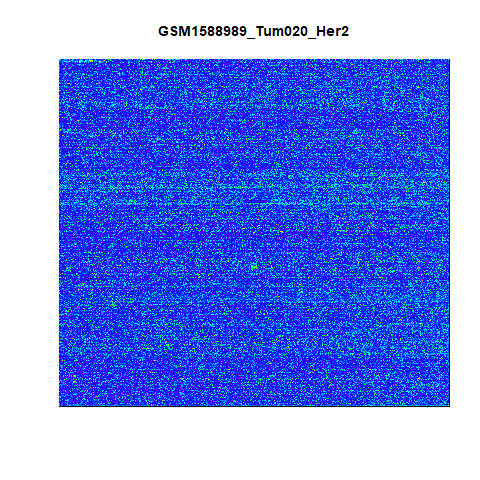
\includegraphics[width=0.5\linewidth]{images/breast_chip_control_example1} 

}

\caption{Working chip of breast cancer microarray GSE65216}\label{fig:unnamed-chunk-1}
\end{figure}

\hypertarget{meansd-plot}{%
\subsubsection{meanSd plot}\label{meansd-plot}}

The meanSd plot shows the standard deviation of the vsn normalized data,
across all samples, plotted against the mean. Here, the logarithmic
transformation consists with the base of 2.

\begin{figure}

{\centering 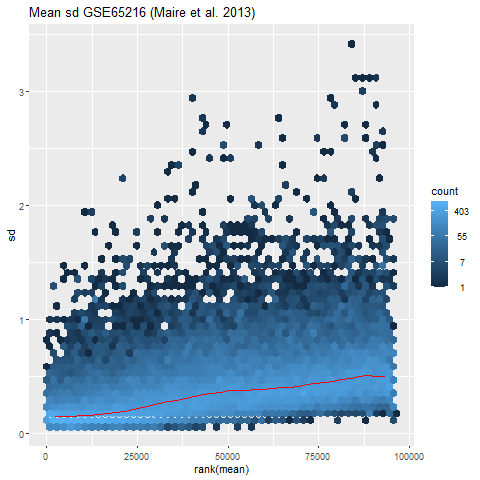
\includegraphics[width=0.5\linewidth]{images/breast_meansdPlot} 

}

\caption{meanSD plot of breast cancer microarray GSE65216}\label{fig:unnamed-chunk-2}
\end{figure}

\hypertarget{boxplots-before-and-after-normalisation}{%
\subsubsection{Boxplots before and after
normalisation}\label{boxplots-before-and-after-normalisation}}

It is clearly visible, that the differences in intensities between
arrays is strongly reduced after normalisation. Also the boxplots only
show little fluctuation in gene expression for the 20 arrays after
normalisation. This means all chips adjudted through vsnrma
normalisation

\begin{figure}

{\centering 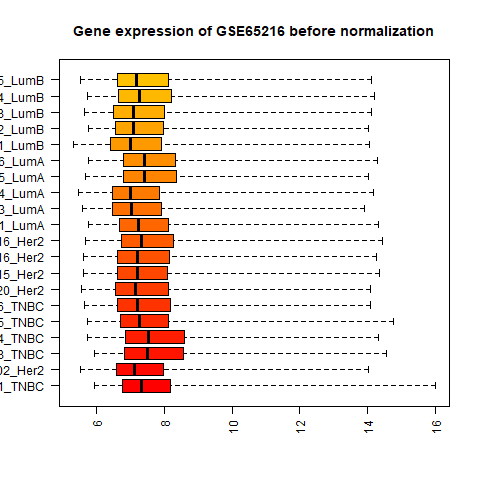
\includegraphics[width=0.5\linewidth]{images/breast_box_bfnorm} 

}

\caption{Boxplots before and after normalisation breast cancer GSE65216}\label{fig:Boxplots - breast qc-1}
\end{figure}
\begin{figure}

{\centering 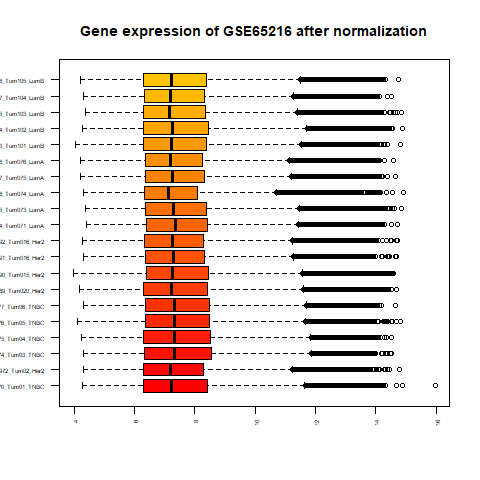
\includegraphics[width=0.5\linewidth]{images/breast_box_afnorm} 

}

\caption{Boxplots before and after normalisation breast cancer GSE65216}\label{fig:Boxplots - breast qc-2}
\end{figure}

\hypertarget{density-function}{%
\subsubsection{Density function}\label{density-function}}

\begin{figure}

{\centering 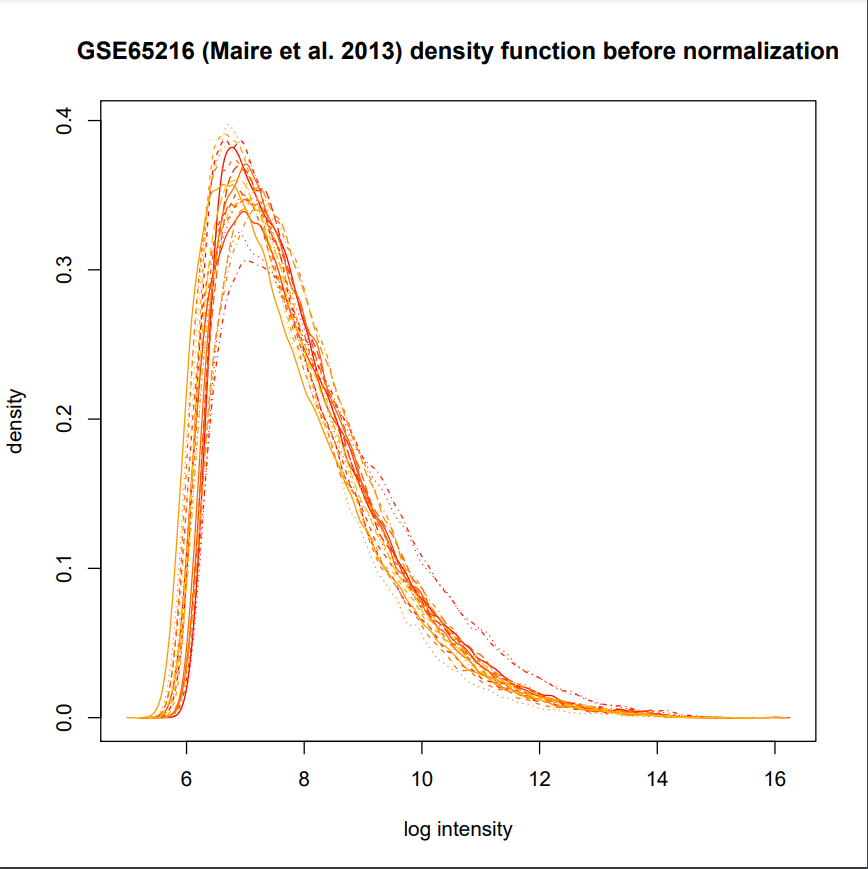
\includegraphics[width=0.5\linewidth]{images/breast_dflog_bfnorm} 

}

\caption{Density functions before and after normalisation breast cancer GSE65216}\label{fig:Density - breast qc-1}
\end{figure}
\begin{figure}

{\centering 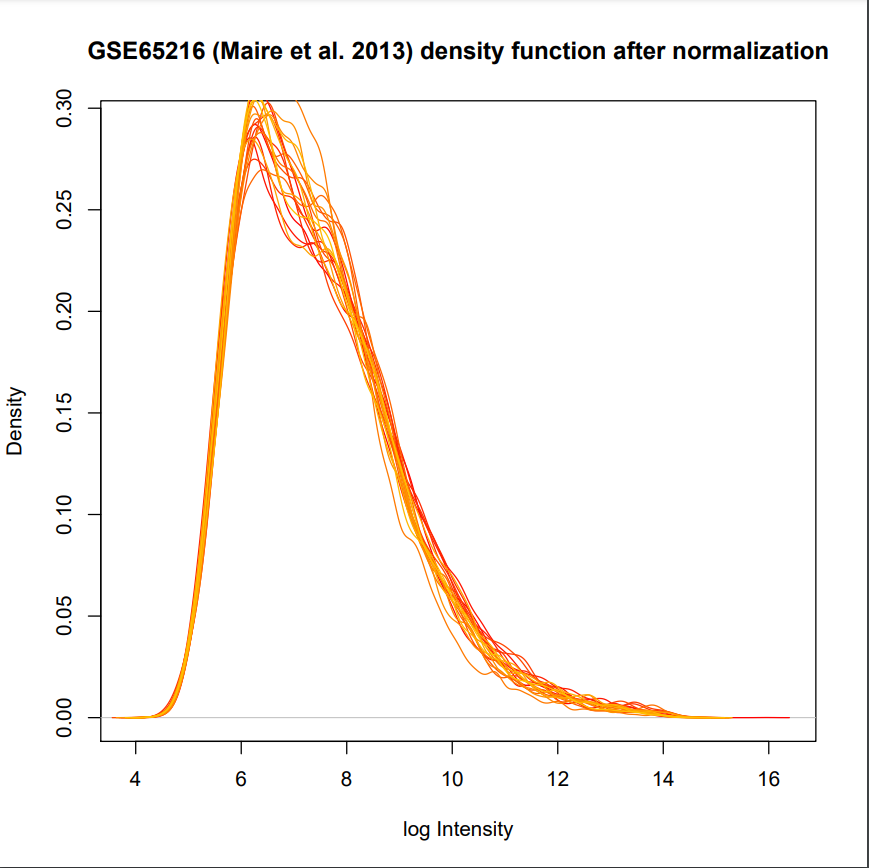
\includegraphics[width=0.5\linewidth]{images/breast_dflog_afnorm} 

}

\caption{Density functions before and after normalisation breast cancer GSE65216}\label{fig:Density - breast qc-2}
\end{figure}

\hypertarget{rna-degeneration-plot}{%
\subsubsection{RNA degeneration plot}\label{rna-degeneration-plot}}

---\textgreater{} MUSS NOCH GSE NUMMER IN PLOT ÜBERSCHRIFT EINGEFÜGT
WERDEN \#\#\# Scatter plots We plotted each sample against the following
sample. If the scattered points deviate strongly from the red line, like
for example forming a banana-like shape, then one of the respective
chips for the sample must be broken. However this seems not to be the
case here.

\begin{figure}

{\centering 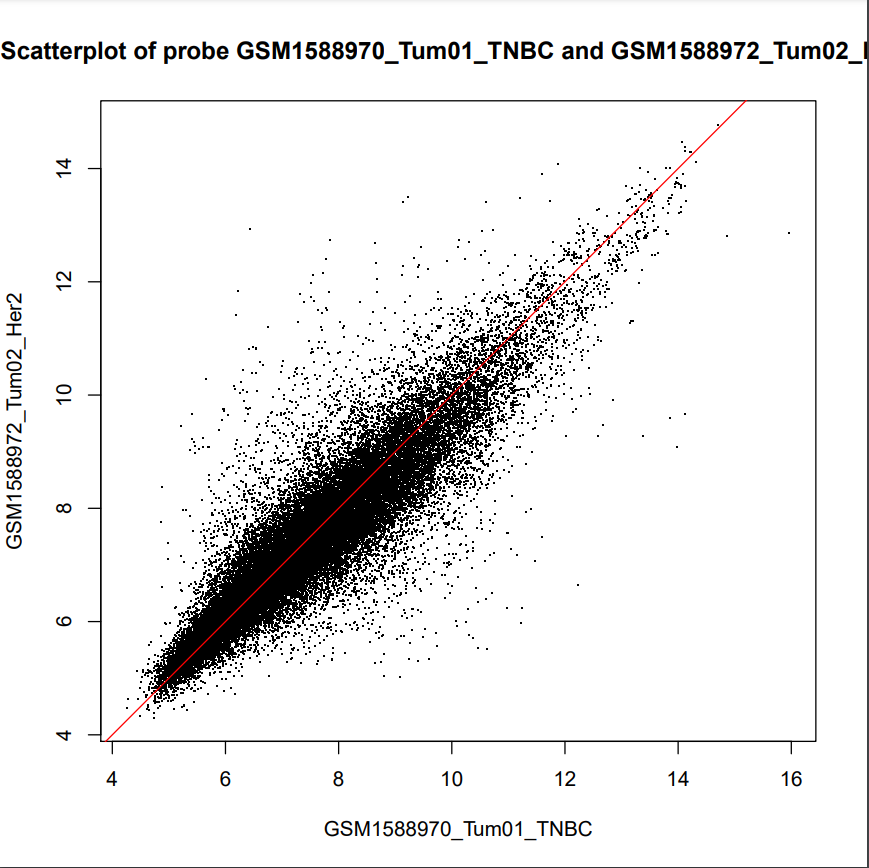
\includegraphics[width=0.5\linewidth]{images/breast_scatter_example1} 

}

\caption{Example of scatter plot breast cancer GSE65216}\label{fig:Scatter plot - breast qc}
\end{figure}

\hypertarget{quality-control---gse149507-lung-cancer}{%
\subsection{2.2 Quality control - GSE149507 lung
cancer}\label{quality-control---gse149507-lung-cancer}}

\hypertarget{single-chip-control-1}{%
\subsubsection{Single chip control}\label{single-chip-control-1}}

\hypertarget{meansd-plot-1}{%
\subsubsection{meanSd plot}\label{meansd-plot-1}}

\hypertarget{boxplots-before-and-after-normalisation-1}{%
\subsubsection{Boxplots before and after
normalisation}\label{boxplots-before-and-after-normalisation-1}}

\hypertarget{density-function-1}{%
\subsubsection{Density function}\label{density-function-1}}

\hypertarget{rna-degeneration-plot-1}{%
\subsubsection{RNA degeneration plot}\label{rna-degeneration-plot-1}}

\hypertarget{scatter-plots}{%
\subsubsection{Scatter plots}\label{scatter-plots}}

The carcinoma tissue sample of patient number 5 did not show linear
relationship to all of the other samples. Since the samples of dataset
GSE149507 for normal and carcinoma tissue are linked to one patient
each, we consequently replaced the two chips GSM4504109\_SCLC\_05\_ca
and GSM4504110\_SCLC\_05\_ with new 2 new chips out of the gene
expression omnibus. When performing the scatter plot control over again,
there are no discrepancies anymore.

\begin{figure}

{\centering 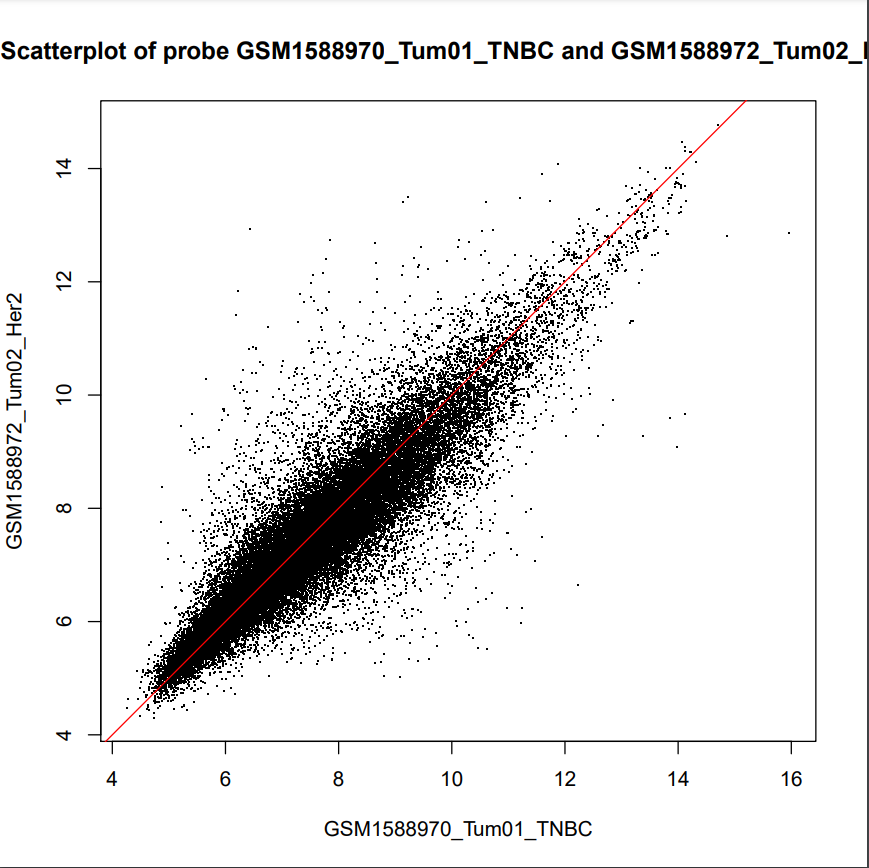
\includegraphics[width=0.5\linewidth]{images/breast_scatter_example1} 

}

\caption{Example of scatter plot breast cancer GSE65216}\label{fig:Broken chip - lung qc}
\end{figure}

\hypertarget{further-data-acquistion}{%
\section{3. Further data acquistion}\label{further-data-acquistion}}

\hypertarget{importing-and-unification-of-tra-data}{%
\subsection{Importing and unification of TRA
data}\label{importing-and-unification-of-tra-data}}

To distinguish between TRA KLK genes and non-TRA KLK genes, we imported
a total of 6 TRA data sets ((Su et al.~2002, 2004), (Roth et al.~2008),
(Lattin et al.~2006), (human GTEX data 2015), (Uhlén et al.~2015)). Also
below you can see an overview of the tissues that display TRAs in the
context of the whole data set.

\hypertarget{expression-analysis}{%
\section{4. Expression Analysis}\label{expression-analysis}}

\hypertarget{extraction-of-klk-and-klk-tra-genes}{%
\subsection{Extraction of KLK and KLK TRA
genes}\label{extraction-of-klk-and-klk-tra-genes}}

With the unified TRA data set Union.TRA, it is possible to extract all
KLKs that are tissue-restricted by their transcript number.

\hypertarget{breast-cancer-gse65216-maire-et-al.-2013}{%
\subsection{4.2 Breast cancer GSE65216 (Maire et
al.~2013)}\label{breast-cancer-gse65216-maire-et-al.-2013}}

The breast cancer microarray GSE65216 (Maire et al.~2013) chips consists
of 20 samples. The samples are all breast cancer tissue differentiated
by four types of mutations. These are Triple negative breast cancer
(TNBC), Her2, Luminal A and Luminal B.\\
\#\#\# Clean up identical isoforms Having a look onto the data set
itself, it is noticeable, that some of the Expression values of the KLK
isoforms in our microarray are exactly identical. These identical
isoforms will be cleared out of our data frame. This is easily done by
performing correlation, here the pearson correlation, between all KLK
genes in a diagonal matrix. If the correlation yields a value of 1 then
the two gene isoforms are the same and the latter one of both will be
removed. Furthermore, the KLKs are sorted after their names in ascending
order for the visualization via the boxplots. In the end, 39 identical
isoforms are removed, whereas a total of 73 KLK transcripts for the 15
KLK genes are being kept. Out of the 73 isoforms, 63 are TRAs, while
only 10 are regarded as tissue restricted.

\hypertarget{visualization-of-gene-expression}{%
\subsubsection{Visualization of gene
expression}\label{visualization-of-gene-expression}}

\hypertarget{overview-gene-expression}{%
\paragraph{Overview gene expression}\label{overview-gene-expression}}

Since the data is vsnrma normalized, the median does not fluctuate too
much for all samples. The lowest gene expression value is about 5 while
the highest gene expression value is around 15. Due to the logarithmic
scale with a base of 2, a log-fold change of +1 represents a two times
as high gene expression.

\begin{Shaded}
\begin{Highlighting}[]
\NormalTok{gene.summary <-}\StringTok{ }\ControlFlowTok{function}\NormalTok{(x)\{}
 \KeywordTok{round}\NormalTok{(}\KeywordTok{apply}\NormalTok{(x, }\DecValTok{2}\NormalTok{, summary), }\DataTypeTok{digits =} \DecValTok{2}\NormalTok{)}
\NormalTok{\}}
\KeywordTok{gene.summary}\NormalTok{(breastExprs)}
\end{Highlighting}
\end{Shaded}

\begin{verbatim}
##         GSM1588970_Tum01_TNBC GSM1588972_Tum02_Her2 GSM1588974_Tum03_TNBC
## Min.                     5.57                  5.56                  5.79
## 1st Qu.                  6.76                  6.78                  6.80
## Median                   7.50                  7.49                  7.50
## Mean                     7.81                  7.78                  7.81
## 3rd Qu.                  8.54                  8.47                  8.49
## Max.                    15.95                 14.87                 14.28
##         GSM1588975_Tum04_TNBC GSM1588976_Tum05_TNBC GSM1588977_Tum06_TNBC
## Min.                     5.82                  5.55                  5.63
## 1st Qu.                  6.79                  6.83                  6.81
## Median                   7.48                  7.57                  7.57
## Mean                     7.80                  7.87                  7.87
## 3rd Qu.                  8.47                  8.62                  8.61
## Max.                    14.28                 14.84                 14.65
##         GSM1588989_Tum020_Her2 GSM1588990_Tum015_Her2 GSM1588991_Tum016_Her2
## Min.                      5.63                   5.58                   5.67
## 1st Qu.                   6.78                   6.84                   6.82
## Median                    7.48                   7.53                   7.55
## Mean                      7.83                   7.88                   7.80
## 3rd Qu.                   8.54                   8.59                   8.47
## Max.                     14.67                  14.59                  14.70
##         GSM1588992_Tum016_Her2 GSM1589064_Tum071_LumA GSM1589065_Tum073_LumA
## Min.                      5.71                   5.65                   5.58
## 1st Qu.                   6.80                   6.84                   6.83
## Median                    7.49                   7.61                   7.58
## Mean                      7.76                   7.85                   7.87
## 3rd Qu.                   8.40                   8.56                   8.59
## Max.                     14.68                  14.77                  14.94
##         GSM1589066_Tum074_LumA GSM1589067_Tum075_LumA GSM1589068_Tum076_LumA
## Min.                      5.51                   5.61                   5.62
## 1st Qu.                   6.81                   6.83                   6.81
## Median                    7.45                   7.52                   7.46
## Mean                      7.70                   7.78                   7.75
## 3rd Qu.                   8.32                   8.44                   8.39
## Max.                     15.05                  14.66                  14.56
##         GSM1589093_Tum101_LumB GSM1589094_Tum102_LumB GSM1589095_Tum103_LumB
## Min.                      5.45                   5.63                   5.65
## 1st Qu.                   6.77                   6.76                   6.77
## Median                    7.53                   7.54                   7.46
## Mean                      7.83                   7.85                   7.80
## 3rd Qu.                   8.58                   8.59                   8.49
## Max.                     14.91                  14.90                  14.88
##         GSM1589097_Tum104_LumB GSM1589098_Tum105_LumB
## Min.                      5.61                   5.54
## 1st Qu.                   6.79                   6.78
## Median                    7.46                   7.52
## Mean                      7.78                   7.81
## 3rd Qu.                   8.43                   8.53
## Max.                     14.49                  14.80
\end{verbatim}

The histogram represent the frequency of the present gene expression in
breast cancer samples. It also shows, that the median gene expression of
KLKs is much lower than the overall median gene expression. This means
that most of the KLK gene expression is normally down-regulated in the
perspective of the whole genome. (Yousef et al.~2004)

\begin{figure}

{\centering 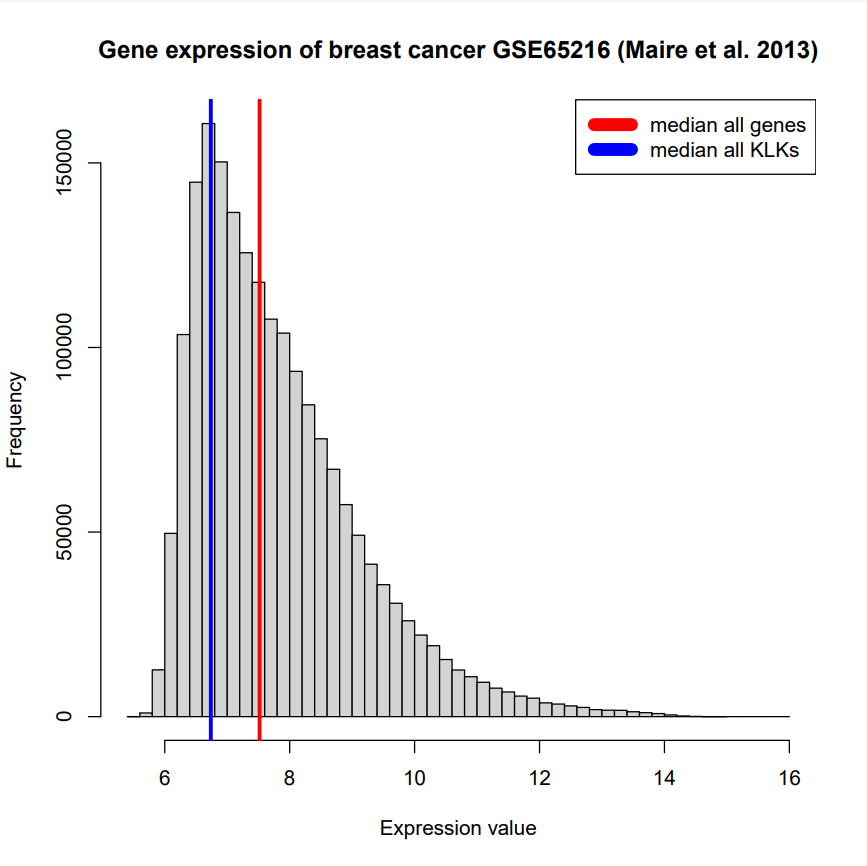
\includegraphics[width=0.5\linewidth]{images/Histogram_breast} 

}

\caption{Histogram of breast cancer gene expression}\label{fig:Histogram - breast }
\end{figure}

\hypertarget{boxplots}{%
\paragraph{Boxplots}\label{boxplots}}

\begin{figure}

{\centering 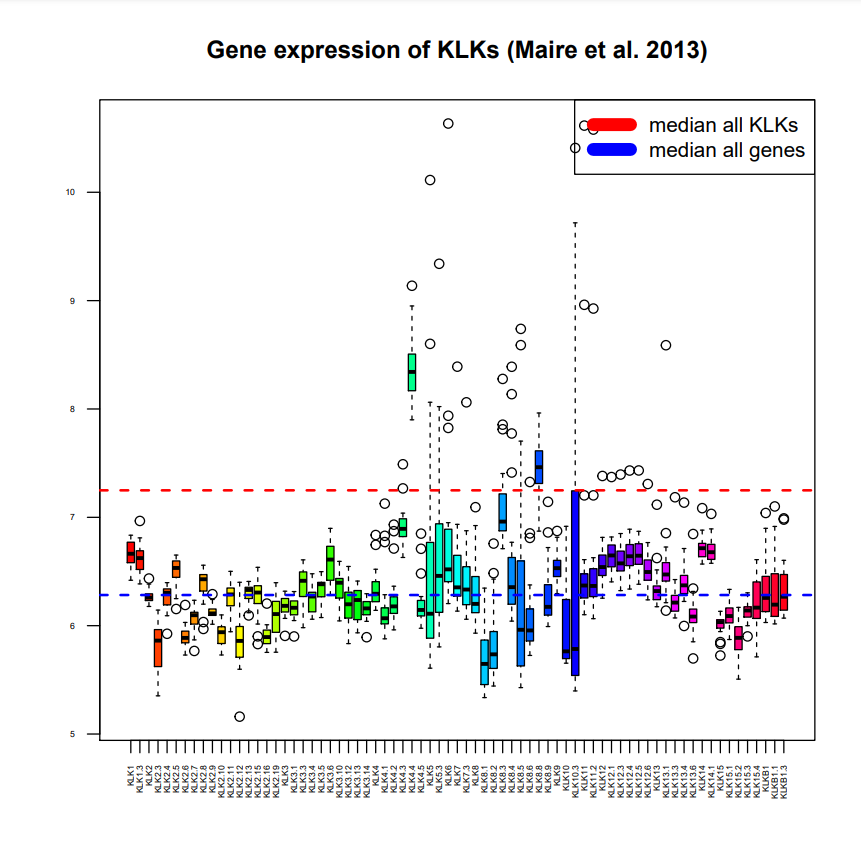
\includegraphics[width=0.5\linewidth]{images/Boxplot_breast} 

}

\caption{Boxplot of KLK gene expression in breast cancer}\label{fig:Boxplot - breast }
\end{figure}

Here, the pattern for the fairly low gene expression of KLKs is also
recognizable. Most of the boxpots of the single KLK gene isoforms are
lower than the median expression of the whole breast cancer genome. Some
KLK isoforms like KLK2.3 are even below a gene expression value of 6, so
KLK isoforms like these are clearly down-regulated. This is compatible
with the finding of Yousef et al.~in which they state an overall
down-regulation of KLK gene expression in breast cancer. There are only
two isoforms that exceed the median of the whole genome expression of
the breast cancer set. These are the isoforms KLK4.4 and KLK8.8.\\
KLK4 gene expression was found by Schmitt et al.~to be up-regulated in
breast cancer tissue as in comparison to healthy breast tissue. This
seems to correspond with the finding shown in the boxplot, but only for
the KLK4.4 isoform. So KLK4.4 needs to be investigated more carefully.
In contrast to that, KLK8 seems to be higher expressed in both normal
and cancer tissue.(Schmitt et al.~2013)

\hypertarget{heatmap}{%
\paragraph{Heatmap}\label{heatmap}}

The dendrogram is the core for the emerging clustering in heatmaps.
Here, clustering is performed after the complete-linkage method.

\begin{figure}

{\centering 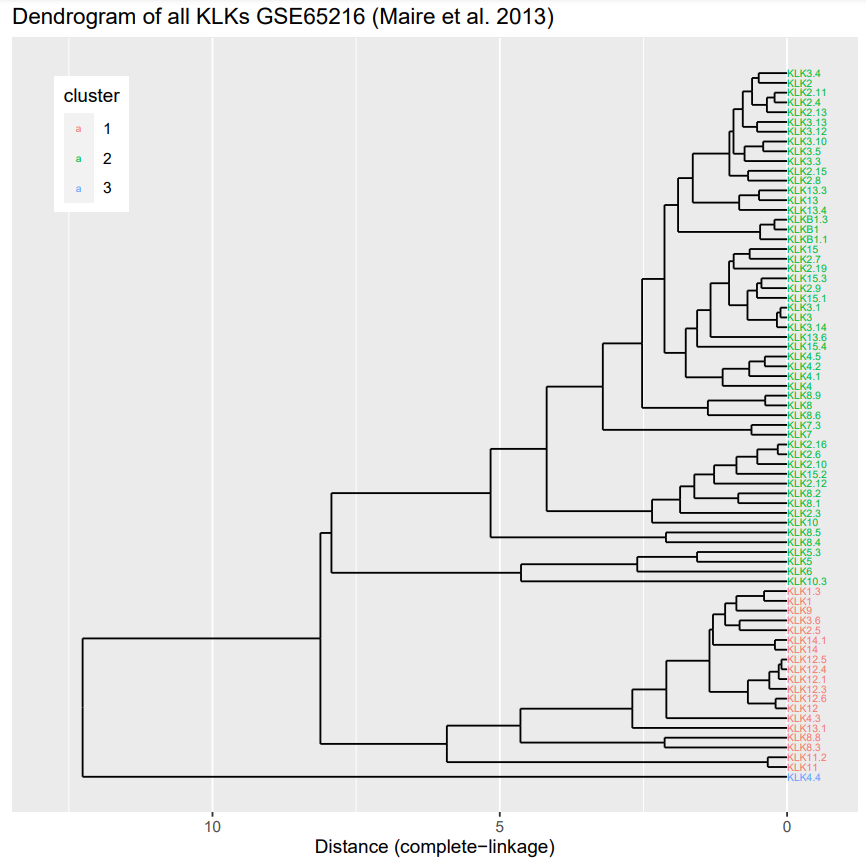
\includegraphics[width=0.5\linewidth]{images/Dendrogram_breast} 

}

\caption{Dendrogram of KLK genes in breast cancer}\label{fig:Dendrogram - breast }
\end{figure}

Interesting in this respect is, that KLK4.4 forms its own branch
independent of all the others. As already shown in the boxplot, KLK4.4
was distinctly up-regulated. Looking onto the other branches of the
dendrogram, it is notable that besides KLK4.4 there are more possible
clusters. To increase the clarity of the heatmap 3 distinguished are
used. Optimal clusters via K-means will still be performed later on.\\

\begin{figure}

{\centering 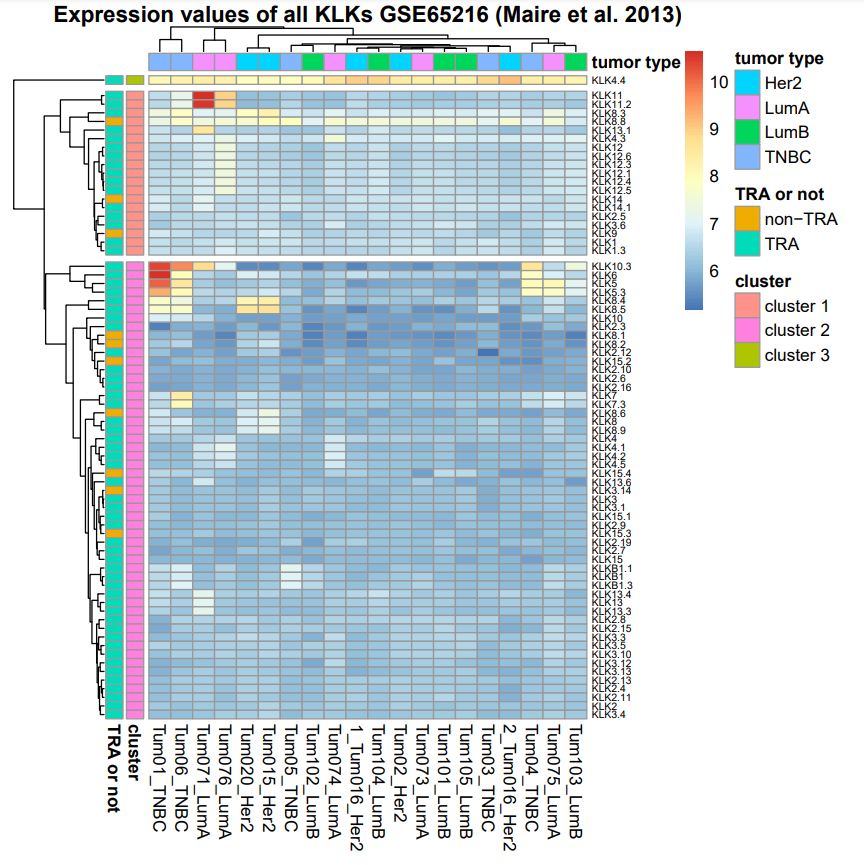
\includegraphics[width=0.5\linewidth]{images/Heatmap_breast} 

}

\caption{Heatmap of KLK gene expression in breast cancer}\label{fig:Heatmap - breast }
\end{figure}

KLK4.4 clearly stands out (cluster 2) with an overall higher expression
across all sample. Furthermore, as it is annotated KLK4.4 belongs to TRA
group. Also in cluster 1 the expression values are higher than in the
third. In addition there are a few samples which seem to have
up-regulated KLK isoforms. For instance, the tumor sample number 1 with
TNBC got one of the highest expression values across the KLKs: KLK10.3,
KLK6 and KLK5.

\hypertarget{pca}{%
\subsubsection{PCA}\label{pca}}

The principal component analysis was conducted over the samples.
Centering was enabled, while scaling was not included, due to the data
being vsnrma normalized.\\

\begin{figure}

{\centering 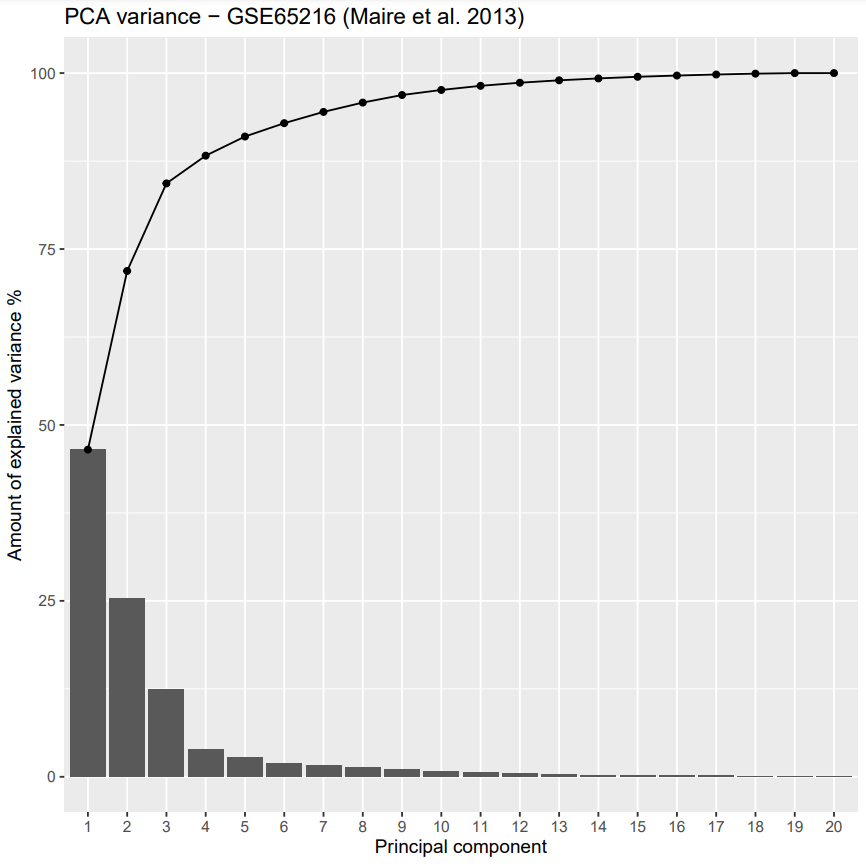
\includegraphics[width=0.5\linewidth]{images/PCA_variance_breast} 

}

\caption{Variance plot of the principal components for breast cancer}\label{fig:PCA variance - breast }
\end{figure}

The cumulative variance shows, that 72\% of the total variance or of the
total information is explained by the first 2 principal components
(PCs). These two PCs are sufficient for the analysis of the distribution
of the breast cancer samples across the loadings of the KLK gene
expression.\\

\begin{figure}

{\centering 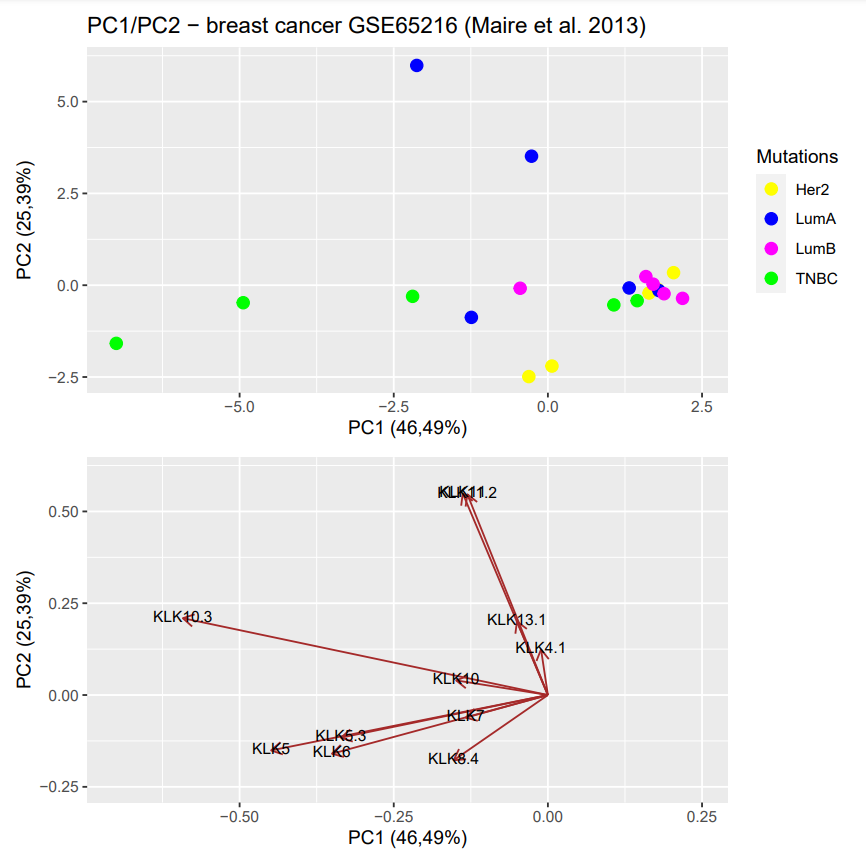
\includegraphics[width=0.5\linewidth]{images/PCAplot_breast} 

}

\caption{PC1 vs. PC2 with their respective loadings for breast cancer}\label{fig:PCA plot - breast }
\end{figure}

The loadings consists of the (SHOW CODE OF THE PCA plot) the top 10 most
differentiated KLK isoforms. This was conducted by adding up the values
of the rotation matrix for each individual KLK isoform. As it is
displayed in Fig. \#NR some samples are more characterized by the
expression of KLK11 and KLK11.2. This is mostly the case for two of the
LumA samples. This was also observable in the heatmap by the higher
expression of KLK11 in the tumor samples 71 and 76. Another result of
the PCA is that TNBC mutations are affected by KLK5 and KLK6 expression,
which is also observable in the heatmap. For the up-regulation of KLK5
and KLK6 for some of the TNBC samples it woud be interesting if this
does also hold truth for a higher sample size. If so, KLK5 and KLK6
expression could presumably be used as biomarker for TNBC breast cancer.
We assume that KLK4.4 is not part of the top 10 loadings, since it is
higher expressed across all tumor samples. \#\#\# K-means clustering
\#\#\# Hypothesis testing

\hypertarget{discussion}{%
\subsubsection{Discussion}\label{discussion}}

\hypertarget{lung-cancer-gse149507-cai-et-al.-2021}{%
\subsection{4.3 Lung cancer GSE149507 (Cai et
al.~2021)}\label{lung-cancer-gse149507-cai-et-al.-2021}}

The lung cancer microarray GSE149507 (Cai et al.~2021) were taken out of
6 patients with small cell lung cancer. The healthy lung tissue is
adjacent to the carcinoma and the data set thereby consists of a total
of 12 samples.

\hypertarget{visualization-of-gene-expression-1}{%
\subsubsection{Visualization of gene
expression}\label{visualization-of-gene-expression-1}}

\hypertarget{overview-gene-expression-1}{%
\paragraph{Overview gene expression}\label{overview-gene-expression-1}}

\begin{figure}

{\centering 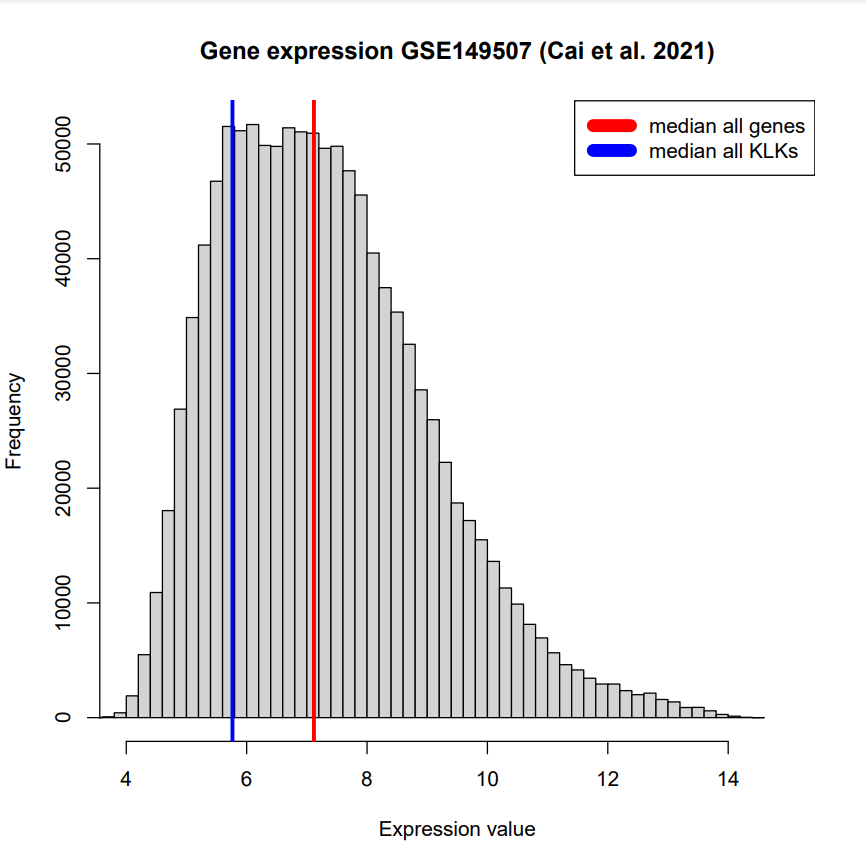
\includegraphics[width=0.5\linewidth]{images/Histogram_lung} 

}

\caption{Histogram of lung cancer gene expression}\label{fig:Histogram - lung }
\end{figure}

\hypertarget{boxplots-1}{%
\paragraph{Boxplots}\label{boxplots-1}}

\begin{figure}

{\centering 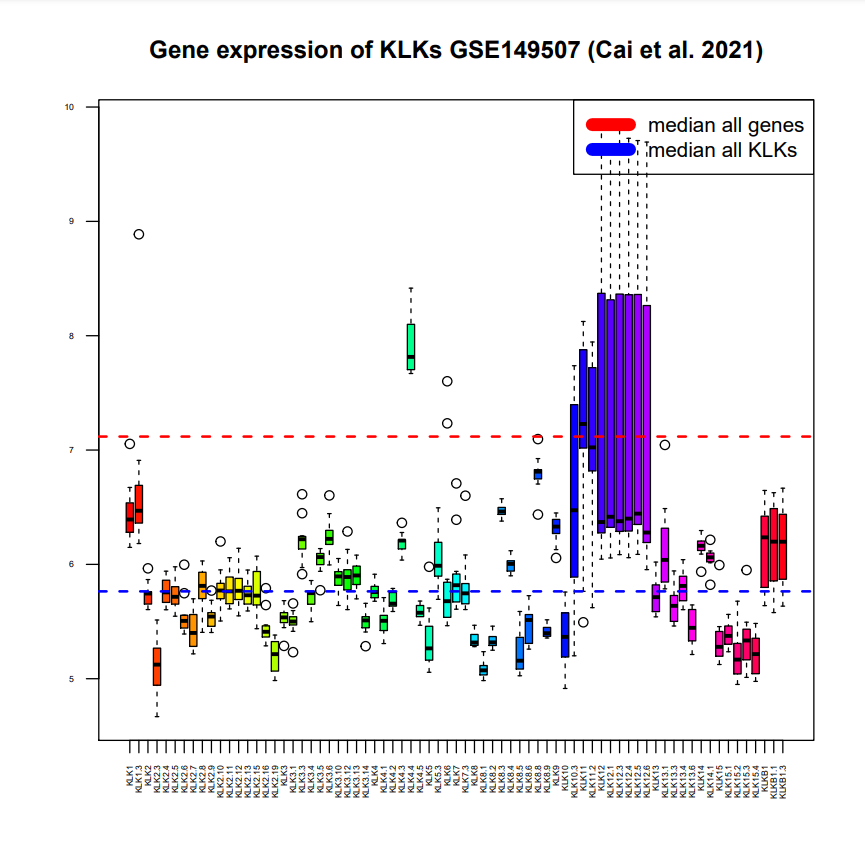
\includegraphics[width=0.5\linewidth]{images/Boxplot_lung} 

}

\caption{Boxplot of KLK gene expression in lung cancer}\label{fig:Boxplot - lung }
\end{figure}

\hypertarget{heatmap-1}{%
\paragraph{Heatmap}\label{heatmap-1}}

\begin{figure}

{\centering 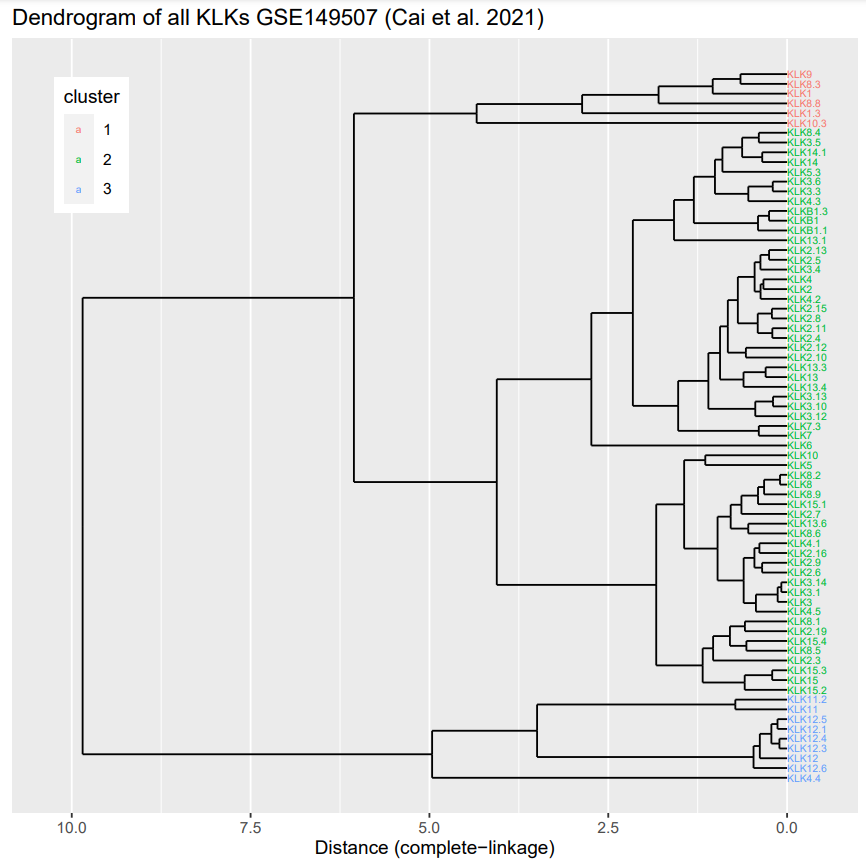
\includegraphics[width=0.5\linewidth]{images/Dendrogram_lung} 

}

\caption{Dendrogram of KLK genes in lung cancer}\label{fig:Dendrogram - lung }
\end{figure}

\begin{figure}

{\centering 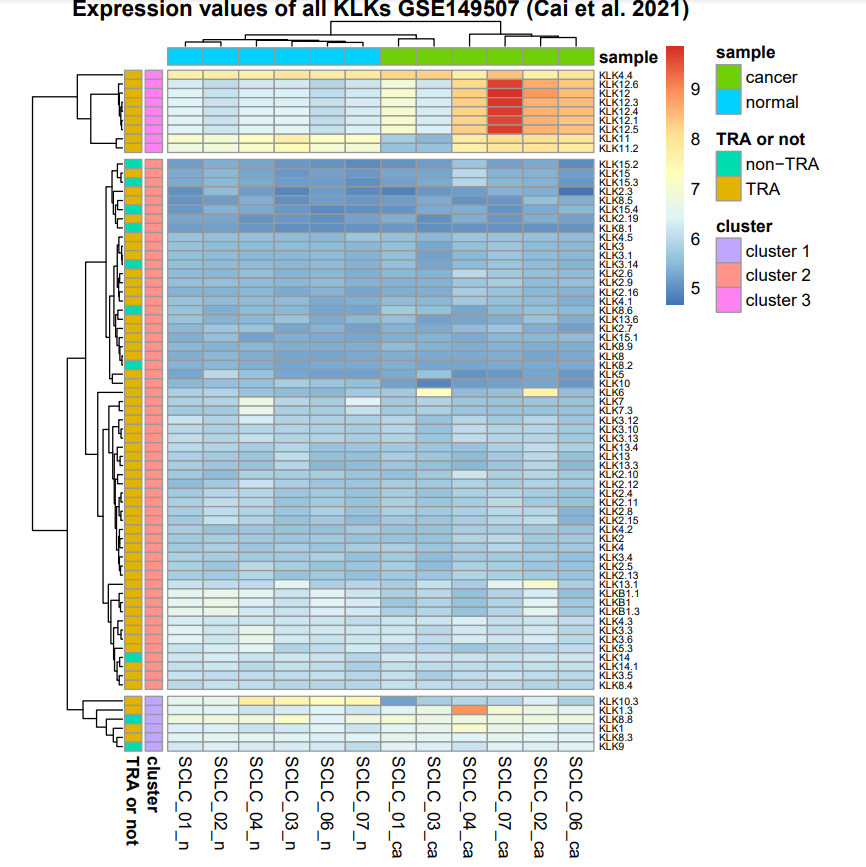
\includegraphics[width=0.5\linewidth]{images/Heatmap_lung} 

}

\caption{Heatmap of KLK gene expression in lung cancer}\label{fig:Heatmap - lung }
\end{figure}

\hypertarget{pca-1}{%
\subsubsection{PCA}\label{pca-1}}

\begin{figure}

{\centering 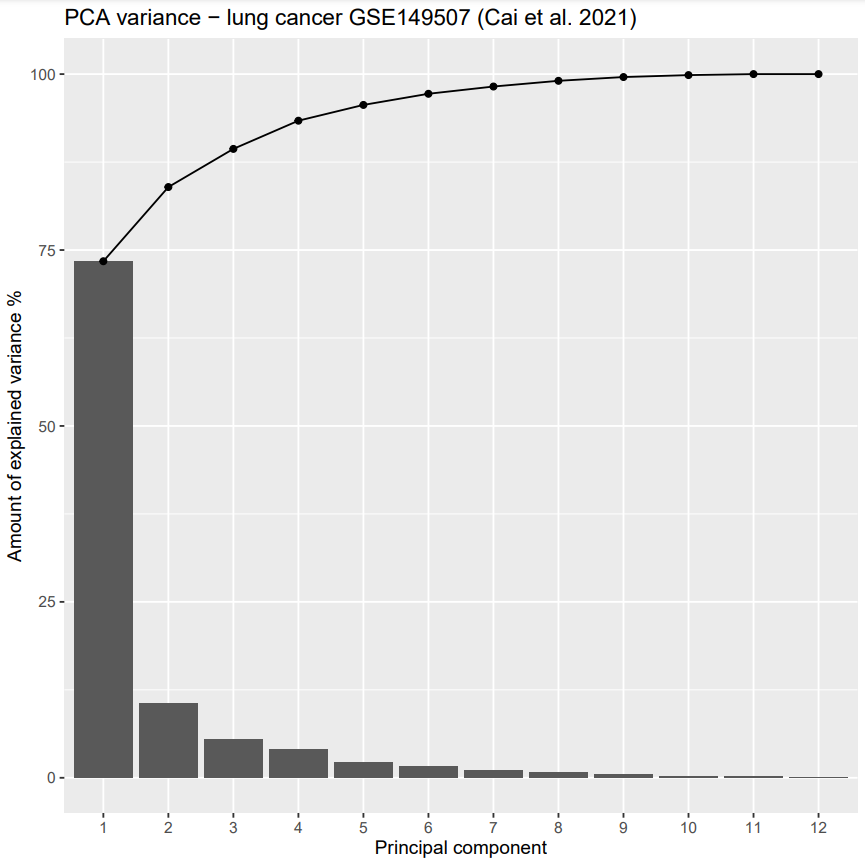
\includegraphics[width=0.5\linewidth]{images/PCA_variance_lung} 

}

\caption{Variance plot of the principal components for lung cancer}\label{fig:PCA variance - lung }
\end{figure}

The cumulative variance shows, that 84\% of the total variance or of the
total information is explained by the first 2 principal components
(PCs). These two PCs are sufficient for the analysis of the distribution
of the breast cancer samples across the loadings of the KLK gene
expression.\\

\begin{figure}

{\centering 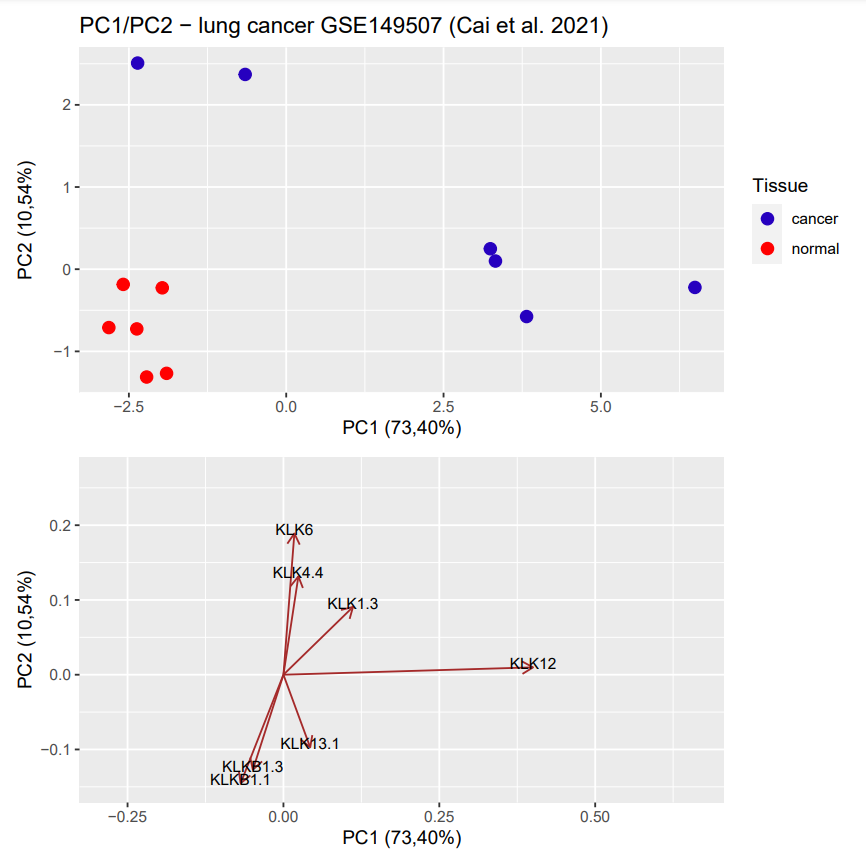
\includegraphics[width=0.5\linewidth]{images/PCAplot_lung} 

}

\caption{PC1 vs. PC2 with their respective loadings for lung cancer}\label{fig:PCA plot - lung }
\end{figure}

\hypertarget{clustering---kmeans}{%
\subsubsection{Clustering - kmeans}\label{clustering---kmeans}}

\hypertarget{hypothesis-testing}{%
\subsubsection{Hypothesis testing}\label{hypothesis-testing}}

The results of the PCA and the k-means indicate that for some KLKs the
expression differs, between the cancerous and normal tissue. Since the
data the data is not normally distributes (QQ-PLOT?) the Wilcoxon
signed-rank test was applied.

\hypertarget{discussion-1}{%
\subsubsection{Discussion}\label{discussion-1}}

\hypertarget{text-k-means-but-for-both}{%
\subsection{Text k means but for both}\label{text-k-means-but-for-both}}

K-means was performed to be able to draw conclusions on characteristics
and the distribution of different Kallikrein genes. Here, we first
determined the optimal number k of clusters in doing a Within Cluster
Sum of Squares -- plot, also called the elbow method. A kink in the
curve of a plot, in which the number k of clusters is plotted against
the within cluster sum of squares, displays the optimal number of k
clusters. Rising numbers of k will not cause a significant decline in
the within cluster sum of squares anymore. For the lung cancer dataset,
the Within Cluster Sum of Squares -- plot predicted an optimal number of
k = 5, so k-means was performed using 5 clusters. The function of
k-means automatically reduces dimensions to 2 if a dataset consists of 3
or more dimensions, so the k-means clustering does not directly cluster
genes of interest according to their expression values, but since
dimension reduction always consists of variables that explain most of
the variance of the data, in this case k-means is still suitable to
compare clusters of Kallikrein genes. K-means performed for the lung
cancer dataset showed an interesting and distinct cluster, which only
consisted of KLK-subtypes of Kallikrein 12. Kallikrein 4.4 was found on
the top left corner. For the breast-cancer dataset, an optimal number of
k = 6 was determined. Here, another cluster was highly distinct,
containing KLK 4.4, which is also examined in the hypothesis testing.
Interestingly, here we could find the cluster containing Kallikrein of
the top right corner, on the opposite side than in the lung cancer
dataset.

\hypertarget{references}{%
\section{References}\label{references}}

\begin{itemize}
\tightlist
\item
  Maire V, Némati F, Richardson M, Vincent-Salomon A et al.~Polo-like
  kinase 1: a potential therapeutic option in combination with
  conventional chemotherapy for the management of patients with
  triple-negative breast cancer. Cancer Res 2013 Jan 15
\item
  Cai L, Liu H, Huang F, Fujimoto J et al.~Cell-autonomous immune gene
  expression is repressed in pulmonary neuroendocrine cells and small
  cell lung cancer. Commun Biol 2021 Mar 9
\item
  Dinkelacker 2019. Chromosomal clustering of tissue restricted
  antigens, Dissertation, University Heidelberg, Germany.
\item
  Dinkelacker 2007. A database of genes that are expressed in a
  tissue-restricted manner to analyse promiscous gene expression in
  medullary thymic epithelial cells. Diplomarbeit,
  Albert-Ludwigs-Universitaet, Freiburg, Germany.
\end{itemize}

\end{document}
